%%% PREAMBLE - Do not touch %%%%%%%%%%%%%%%%%%%%%%%%%%%%%%%%%%%%%%%%%%%%%%%%%%%%%%

\documentclass[10pt,twocolumn,letterpaper]{article}
\usepackage{pdfpages}
\usepackage[utf8]{inputenc}
\usepackage[portuges,brazil,english]{babel}
\usepackage{model}
\usepackage{times}
\usepackage{epsfig}
\usepackage{graphicx}
\usepackage{amsmath}
\usepackage{amssymb}
\usepackage{color}
\usepackage{listings}
\usepackage[pagebackref=true,breaklinks=true,letterpaper=true,colorlinks,bookmarks=false]{hyperref}
%  ABACO -- Conjunto de macros para desenhar o 'abaco
%  Desenho original de Hans Liesenberg
%  Macros de Tomasz Kowaltowski
%  DCC -- IMECC -- UNICAMP
%  Mar,co de 1988  --  Vers~ao 1.0
% Ajustado para LaTeX da SUN -- Mar,co de 1991
% ---------------------------------------------------------
%  Chamada:   \ABACO{d1}{d2}{d3}{d4}{esc}
%             com:  di's -- os quatro d'igitos;
%                   esc  -- fator de escala
% ---------------------------------------------------------
%  DEFINI,C~OES AUXILIARES
% ---------------------------------------------------------
%  Forma o d'igito pequeno (0 ou 1)

\newcommand{\ABACODP}[1]{%
%
\thicklines
%    
\begin{picture}(8,0)
    \ifcase#1{   %  caso 0
       \put(0,0)    {\line(1,0){4}}
       \multiput(5,0)(2,0){2}{\oval(2,4)}}
    \or{         %  caso 1
       \put(2,0)    {\line(1,0){4}}
       \multiput(1,0)(6,0){2}{\oval(2,4)}}
    \fi
\end{picture}
    } % \ABACODP

% Forma o d'igito grande (0 a 4)

\newcommand{\ABACODG}[1]{%
%
\thicklines
%    
\begin{picture}(14,0)
    \ifcase#1{   % caso 0
       \multiput(1,0)(2,0){5}{\oval(2,4)}}
       \put(10,0)   {\line(1,0){4}}
    \or{         % caso 1
       \multiput(1,0)(2,0){4}{\oval(2,4)}}
       \put(8,0)   {\line(1,0){4}}
       \put(13,0)   {\oval(2,4)}
    \or{         % caso 2
       \multiput(1,0)(2,0){3}{\oval(2,4)}
       \put(6,0)   {\line(1,0){4}}
       \multiput(11,0)(2,0){2}{\oval(2,4)}}
    \or{         % caso 3
       \multiput(1,0)(2,0){2}{\oval(2,4)}
       \put(4,0)   {\line(1,0){4}}
       \multiput(9,0)(2,0){3}{\oval(2,4)}}
    \or{         % caso 4
       \put(1,0)  {\oval(2,4)}}
       \put(2,0)   {\line(1,0){4}}
       \multiput(7,0)(2,0){4}{\oval(2,4)}
    \fi
\end{picture}
    } % \ABACODG
       
% Forma um d'igito (0 a 9)

\newcommand{\ABACOD}[1]{%
%
    \ifnum#1>9
       \errmessage{#1: Argumento invalido para ABACO}
    \fi
    \ifnum#1<0
       \errmessage{#1: Argumento invalido para ABACO}
    \fi
%
\begin{picture}(24,0)
%    
    \ifnum#1<5
       \put(16,0) {\ABACODP{0}}
    \else   
       \put(16,0) {\ABACODP{1}}
    \fi
%    
    \ifnum#1<5
       \put(0,0)  {\ABACODG{#1}}
    \else
       \ifcase#1\or \or \or \or
          \or  \put(0,0)  {\ABACODG{0}}
          \or  \put(0,0)  {\ABACODG{1}}
          \or  \put(0,0)  {\ABACODG{2}}
          \or  \put(0,0)  {\ABACODG{3}}
          \or  \put(0,0)  {\ABACODG{4}}
       \fi
    \fi   
\end{picture}
    } % \ABACOD
    
% -------------------------------------------------

%  DEFINI,C~AO PRINCIPAL
    
\newcommand{\ABACO}[5]{%
    \setlength{\unitlength}{#5mm}
%
    \thinlines
%   
\begin{picture}(28,25)
%   
% moldura
%
% externa
%
        \put(0,0)            {\line(0,1){25}}
        \put(0,0)            {\line(1,0){28}}
        \put(28,0)           {\line(0,1){25}}
        \put(0,25)           {\line(1,0){28}}
% interna
        \put(2,2)            {\line(0,1){21}}
        \put(26,2)           {\line(0,1){21}}
        \put(16,2)           {\line(0,1){21}}
        \put(18,2)           {\line(0,1){21}}
        \put(2,2)            {\line(1,0){14}}
%        \put(16,2)           {\line(1,-1){1}}
%        \put(17,1)           {\line(1,1){1}}
        \put(18,2)           {\line(1,0){8}}
        \put(2,23)           {\line(1,0){14}}
%        \put(16,23)          {\line(1,1){1}}
%       \put(17,24)          {\line(1,-1){1}}
        \put(18,23)          {\line(1,0){8}}
%        \put(0,0)            {\line(1,1){2}}
%        \put(0,25)           {\line(1,-1){2}}
%        \put(28,0)           {\line(-1,1){2}}
%        \put(28,25)          {\line(-1,-1){2}}
%
%   
% d'igitos
%
%   
       \put(2,20)  {\ABACOD{#1}}
       \put(2,15)  {\ABACOD{#2}}
       \put(2,10)  {\ABACOD{#3}}
       \put(2,5)   {\ABACOD{#4}}
%      
\end{picture}
    } % \ABACO
    

\usepackage[usenames,dvipsnames]{color}    
\usepackage[usenames,dvipsnames]{color}    
 \lstset{ 
  language=R,                     % the language of the code
  basicstyle=\footnotesize\ttfamily, % the size of the fonts that are used for the code
  numbers=left,                   % where to put the line-numbers
  numberstyle=\footnotesize\color{Blue},  % the style that is used for the line-numbers
  stepnumber=1,                   % the step between two line-numbers. If it's 1, each line
                                  % will be numbered
  numbersep=5pt,                  % how far the line-numbers are from the code
  backgroundcolor=\color{white},  % choose the background color. You must add \usepackage{color}
  showspaces=false,               % show spaces adding particular underscores
  showstringspaces=false,         % underline spaces within strings
  showtabs=false,                 % show tabs within strings adding particular underscores
  frame=single,                   % adds a frame around the code
  rulecolor=\color{black},        % if not set, the frame-color may be changed on line-breaks within not-black text (e.g. commens (green here))
  tabsize=2,                      % sets default tabsize to 2 spaces
  captionpos=b,                   % sets the caption-position to bottom
  breaklines=true,                % sets automatic line breaking
  breakatwhitespace=false,        % sets if automatic breaks should only happen at whitespace
  keywordstyle=\color{RoyalBlue},      % keyword style
  commentstyle=\color{YellowGreen},   % comment style
  stringstyle=\color{ForestGreen}      % string literal style
} 
\cvprfinalcopy % *** Uncomment this line for the final submission
\def\httilde{\mbox{\tt\raisebox{-.5ex}{\symbol{126}}}}
\ifcvprfinal\pagestyle{empty}\fi

\newcommand{\TODO}[1]{TODO: #1}
\newcommand{\CITEONE}[2]{\mbox{#1 \cite{#2}}}
\newcommand{\CITETWO}[3]{\mbox{#1 and #2 \cite{#3}}}
\newcommand{\CITEN}[2]{\mbox{#1 et al. \cite{#2}}}

%%% Report beginning %%%%%%%%%%%%%%%%%%%%%%%%%%%%%%%%%%%%%%%%%%%%%%%%%%%%%%%%%%%%%%
\begin{document}
%%% Title and authors %%%%%%%%%%%%%%%%%%%%%%%%%%%%%%%%%%%%%%%%%%%%%%%%%%%%%%%%%%%%
\title{Child stuntedness}
\author{Fabio Fogliarini Brolesi\thanks{Is with the Institute of Computing, University of Campinas (Unicamp). \textbf{Contact}: \tt\small{fabio$\Theta$fabio.mat.br}}\\
Francis Luz\thanks{Is with the Institute of Computing, University of Campinas (Unicamp). \textbf{Contact}: \tt\small{francis$\Theta$francisluz.com}}
}

%\tableofcontents
%\listoffigures

%%% Abstract %%%%%%%%%%%%%%%%%%%%%%%%%%%%%%%%%%%%%%%%%%%%%%%%%%%%%%%%%%%%%%%%%%%%%
\maketitle
\begin{abstract}
Abstract goes here.
\end{abstract}

\section{Stunting}
\subsection{Definition}
According to \cite{Lewit}, ``Growth stunting is defined by comparing measurements of children's heights to the NCHS\footnote{National Center for Health Statistics} growth reference population: children who fall below the fifth percentile of the reference population in height for age are defined as stunted, regardless of the reason for their shortness. As an indicator of nutritional status, comparison of children's measurements with growth reference curves may be used differently for populations of children than for individual children. The fact that an individual child falls below the fifth percentile for height for age on a growth reference curve may reflect normal variation in growth within a population: the individual child may be short simply because both his parents were short and not because of inadequate nutrition. However, if substantially more than 5\% of an identified child population have height for age that is less than the fifth percentile on the reference curve, then the population is said to have a higher-than-expected prevalence of stunting, and inadequate nutrition is generally the first cause considered."

\subsection {Causes}

Inadequate nutrition is just one of several causes of growth stunting. Other contributors to stunting include chronic or recurrent infections, sometimes in combination with intestinal parasites. The prevalence of growth stunting, particularly among children under two years of age, can also reflect the prevalence of low birth weight in a population. Finally, in rare cases, growth stunting may reflect extreme psychosocial stress without nutritional deficiencies.

The contributions of each of these causes to the growth stunting prevalence rate are only partly understood. One study concluded that from 20\% to 40\% of the prevalence of growth stunting in the first two years of life can be attributed to low birth weight. However, inadequate nutrition may still be implicated because some low weight births may be due to maternal nutritional deficiencies during pregnancy.

Just as low birth weight and nutritional deficiencies are interrelated, so also are inadequate nutrition and the chronic or recurrent infections that are believed to contribute to growth stunting. There is evidence that even mild nutritional deficits can alter the immune response in children, before clinical signs of malnutrition occur, and that nutritional deficiencies during pregnancy can impair the infant's immune response after birth. Thus, the reasons for any given child's growth impairment may be complex. However, inadequate nutrition is a common theme that suggests a key focus for a policy response to the problem of growth stunting.



\subsection{Consequences}

Children who suffer from growth retardation as a result of poor diets or recurrent infections tend to be at greater risk for illness and death. Stunting is the result of long-term nutritional deprivation and often results in delayed mental development, poor school performance and reduced intellectual capacity. This in turn affects economic productivity at national level. Women of short stature are at greater risk for obstetric complications because of a smaller pelvis. Small women are at greater risk of delivering an infant with low birth weight, contributing to the intergenerational cycle of malnutrition, as infants of low birth weight or retarded intrauterine growth tend be smaller as adults.

\subsection{Measuring stunting}

Several important age-related differences and discontinuities in the reference growth curves are used to measure stunting. First, for children less than 24 months of age, growth is determined by measuring the length of a recumbent child. After 24 months, growth is determined by measuring the height of a standing child. Because length and height measurements are not equivalent, there is a natural discontinuity between growth curves for children below and above 24 months of age.

\begin{figure}
\begin{center}
	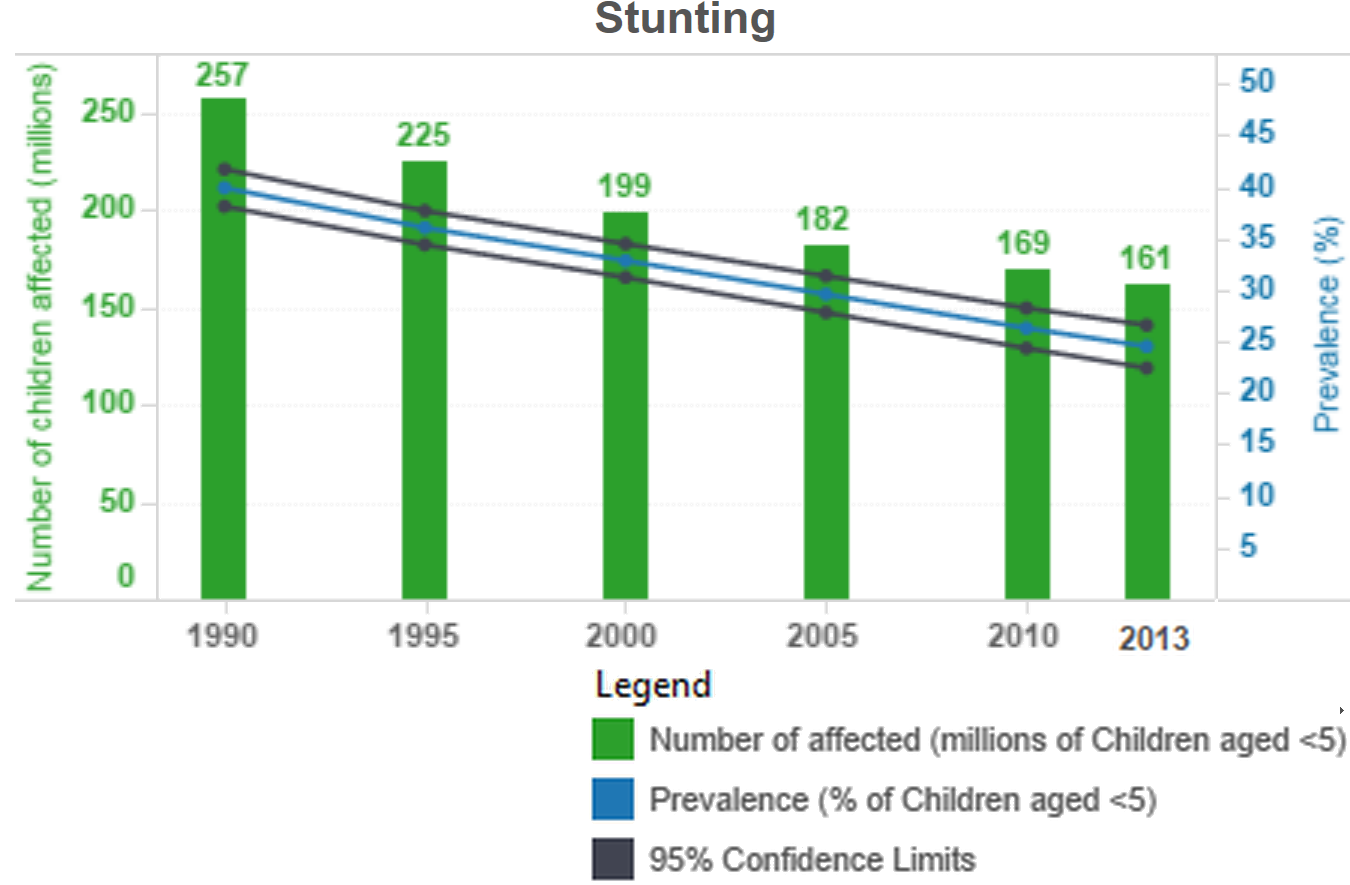
\includegraphics[width=0.99\columnwidth]{pics/unicef01}
	\caption{Child malnutriotion trend for stunting (According to \cite{Unicef}).\label{fig:unicef01}}   
\end{center} 
\end{figure}   

\begin{figure*}
\begin{center}
	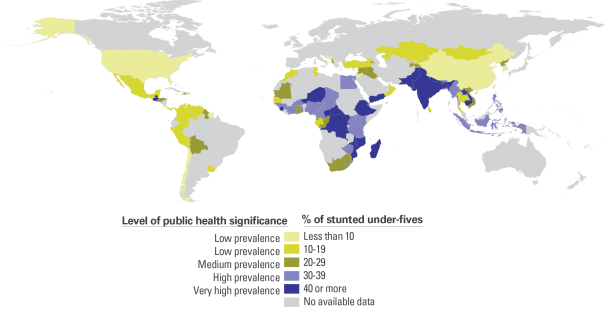
\includegraphics[width=0.99\textwidth]{pics/unicef02}
	\caption{Undernutrition contributes to half of all deaths in children under 5 and is widespread in Asia and Africa
Percentage of under-five children who are stunted, 2008 - 2013).\label{fig:unicef02}}   
\end{center} 
\end{figure*}   

The WHO\footnote{World Health Organization} uses to classify stunting as height for age $< -2$ SD\footnote{standard deviations} of the WHO Child Growth Standards median (measurement charts of girls and boys are at the end of this document).

\section{Problem statement}

% Using the description 1
Our goal is to determine a combination of early measures that would be a good predictor for birth weight. In pursuit of this goal, we have collected time series data from ultrasounds on pregnant mothers. We would like you to use this data to predict a child’s birth weight and birth date (days from pregnancy start).

For each fetus given sex, status, and multiple ultrasound measurements(columns 5-12) during the pregnancy (time being the variable t.ultsnd). The data from the repeated ultrasounds provides a small time series that can be used for predicting the birth weight and day.

For each prediction $(b_i, w_i)$, the error from the true birth date and birth weight will be measured as the squared Mahalanobis distance,

\begin{equation}
e_i = (b_i - b_{0i}, w_i - w_{0i})^TS^{-1}(b_i - b_{0i}, w_i - w_{0i})'
\label{eq:Mahalanobis}
\end{equation}
where $S^{-1}$ is the inverse of the sample covariance matrix calculated on the complete dataset.

\begin{equation}
S^{-1} = \left( \begin{array}{cc}
3554.42 & -328.119 \\
-328.119 &  133.511 
\end{array} \right)
\label{eq:S1}
\end{equation}

Scores will be calculated as a generalized R2 measure of fit. This is calculated as follows. The total sum of errors for the submission will be calculated as $SSE = \sum(e_i)$.

A baseline sum of squared error will be calculated by predicting the sample means for each fetus, that is the mean values of b and w for the current training set,

\begin{equation}
e_{0i} = (\bar{b} - b_{0i}, \bar{w} - w_{0i})S^{-1}(\bar{b} - b_{0i}, \bar{w} - w_{0i})' 
\label{eq:e0i}
\end{equation}

$$SSE_0 = \sum(e_{0i})$$



\section{Charts}
The charts below are from CDC\footnote{Center for Disease Control and Prevention} website and given the default curves of growth for girls and boys from the birth to 24 months.
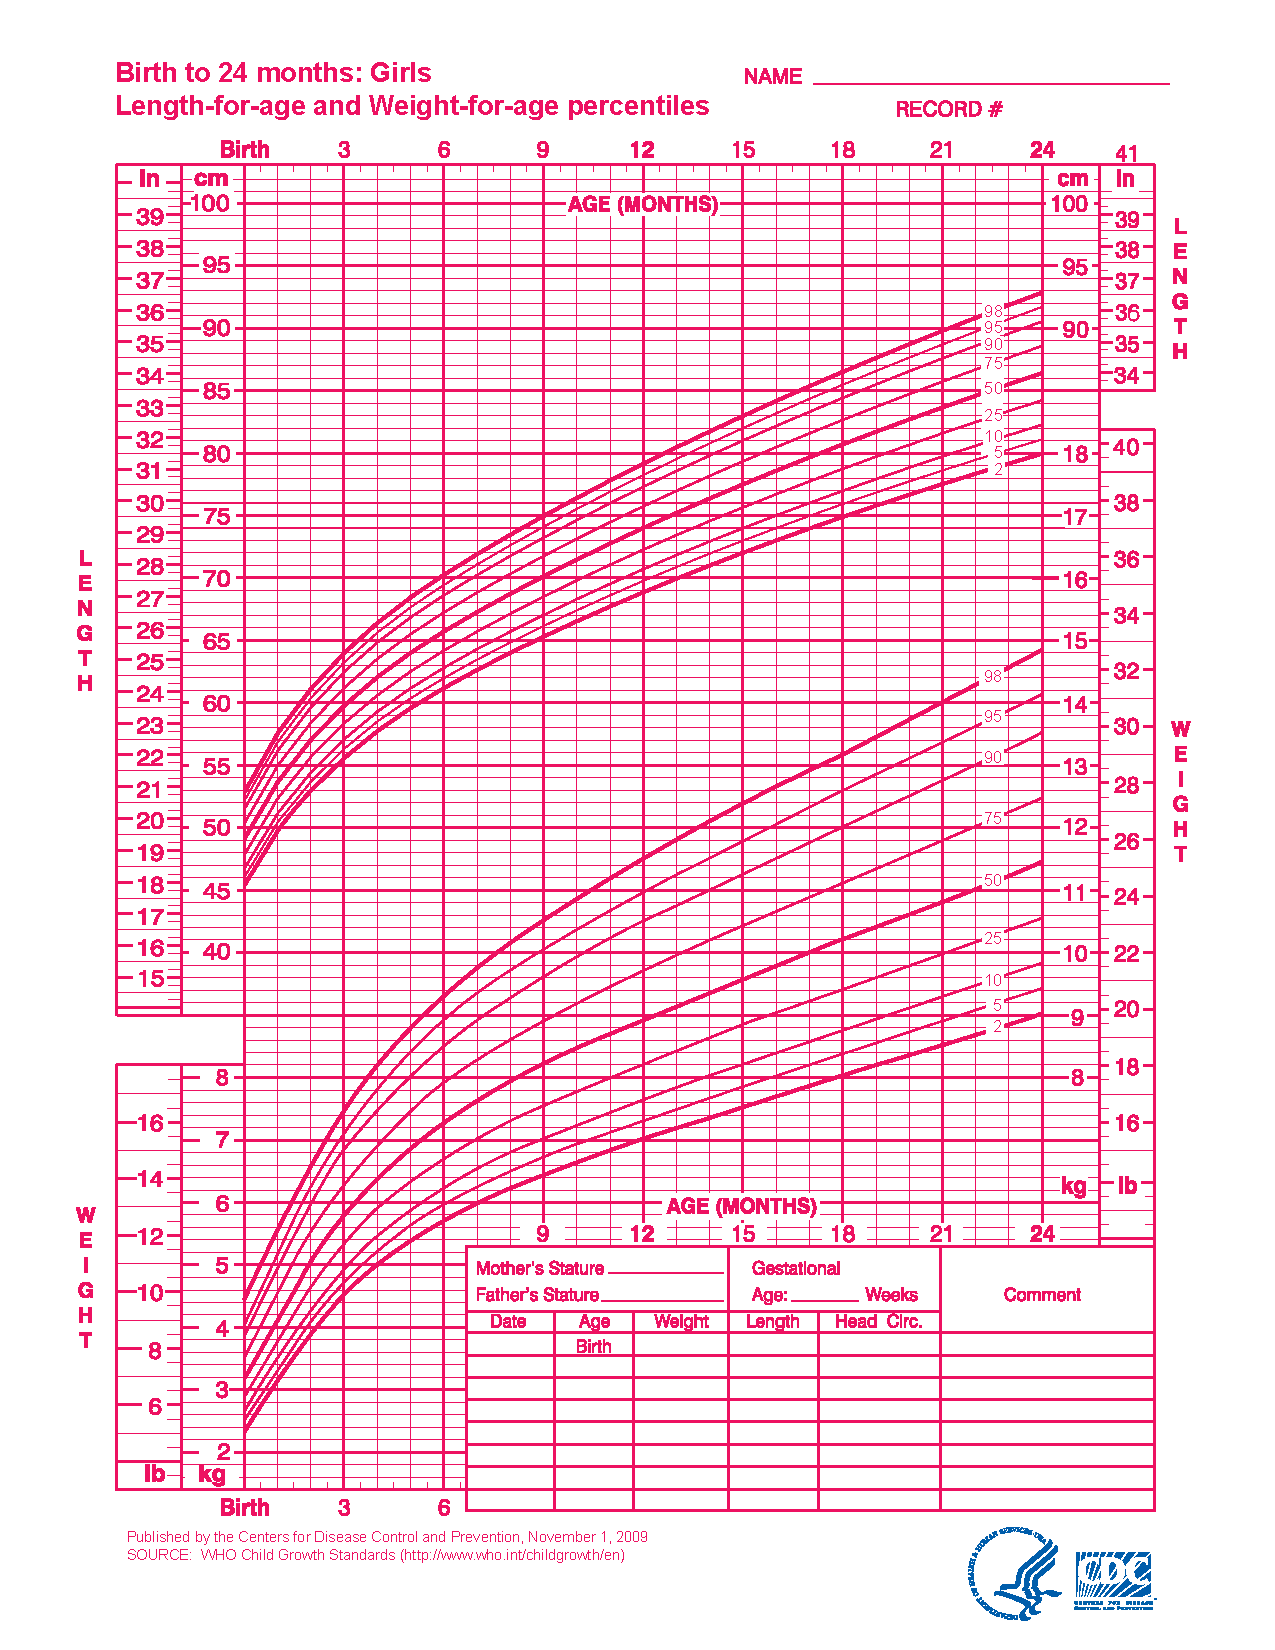
\includepdf[scale=0.8,pages={1}]{pdf/grchrt_girls_24lw_9210.pdf}
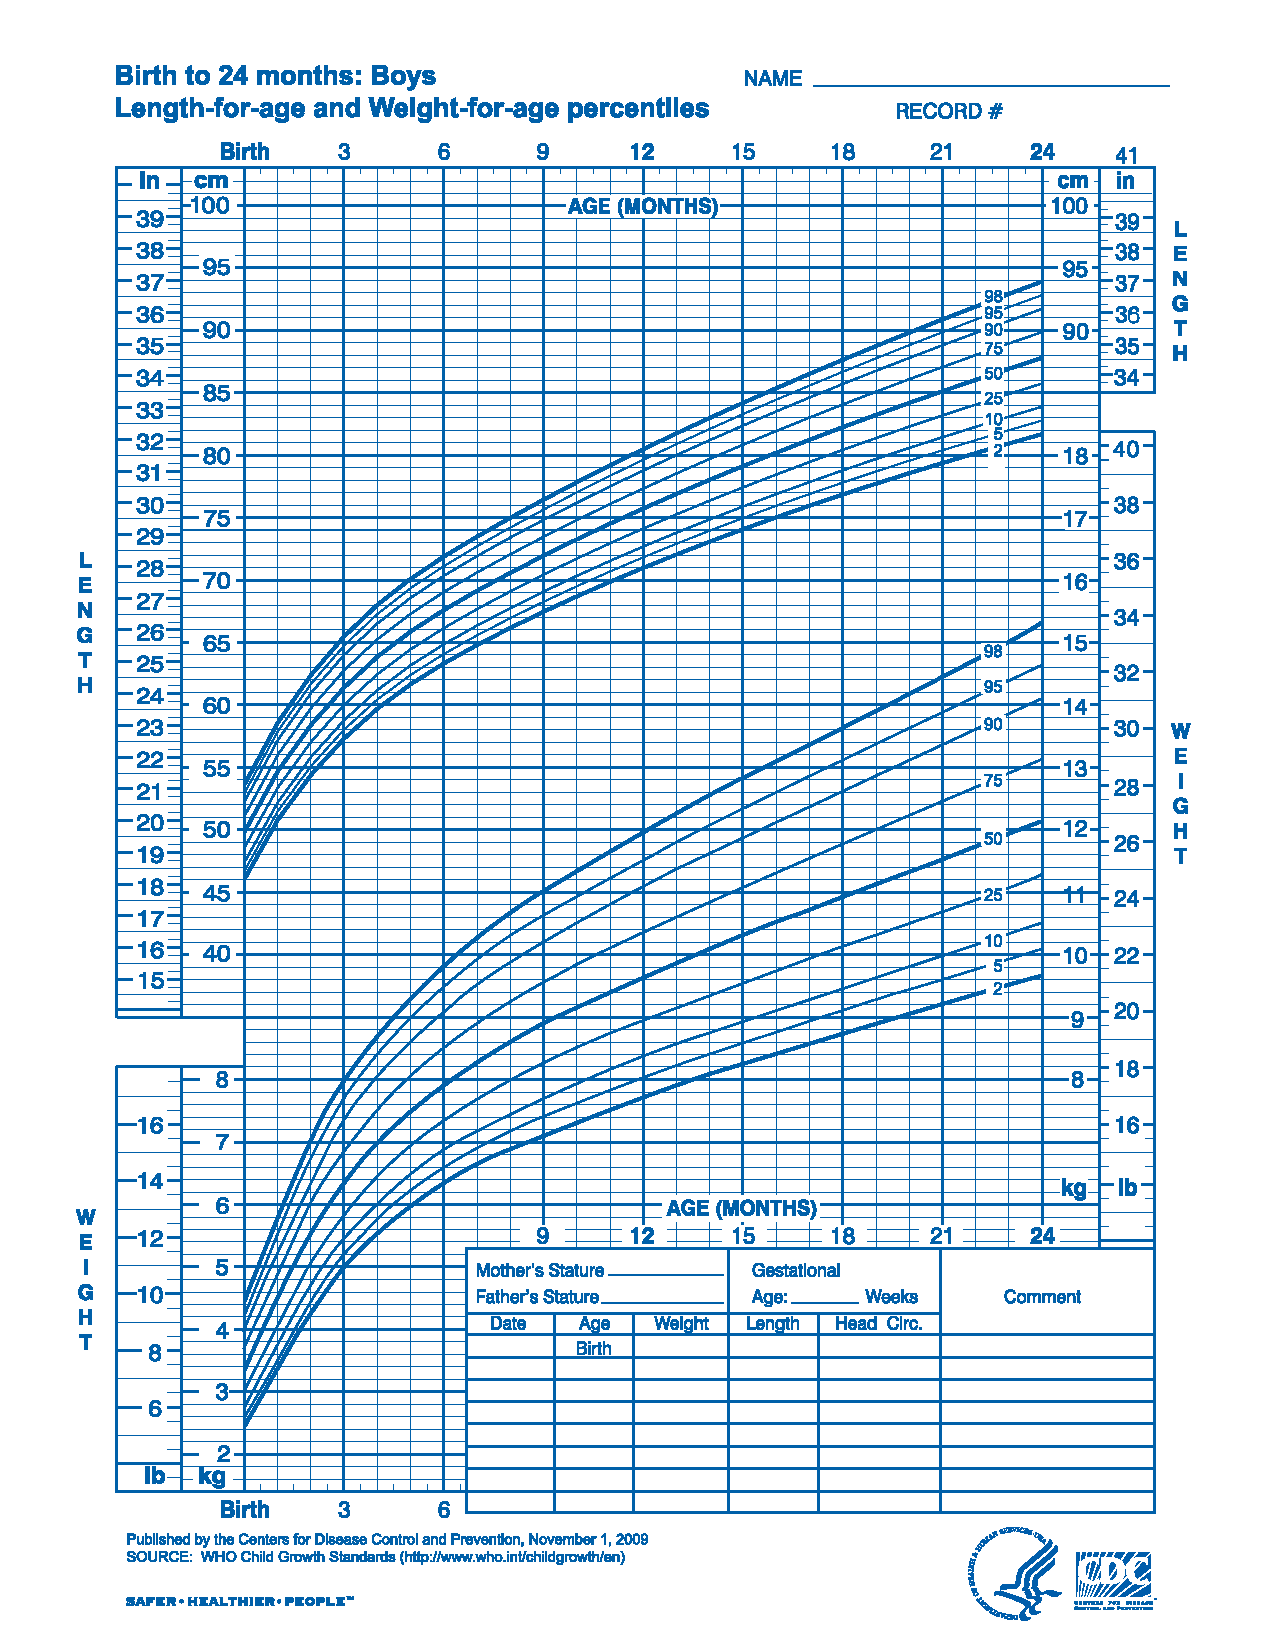
\includepdf[scale=0.8,pages={1}]{pdf/grchrt_boys_24lw_100611.pdf}


%%% References %%%%%%%%%%%%%%%%%%%%%%%%%%%%%%%%%%%%%%%%%%%%%%%%%%%%%%%%%%%%%%%%%%%
\nocite{*}
{\small
\bibliographystyle{unsrt}
\bibliography{refs}
}
\end{document}